\documentclass{article}
\usepackage[utf8]{inputenc}
\usepackage{amsmath}
\usepackage{amssymb}
\usepackage{changepage}
\usepackage{graphicx}
\title{Homework 2 Theory \& Writeup}
\author{Michael Tang}
\date{due May 2, 2019}
\begin{document}
\maketitle
\begin{adjustwidth}{-2cm}{-2cm}
\section{Theory}
\subsection{Exercise 25}
No. L1 requires that every method call has its response immediately after. Essentially, changes done by method must be nonoverlapping and sequential by time. Sequential consistency only requires that method calls appear to execute in a sequential order. This is a looser requirement that doesn't regard time intervals.

\subsection{Exercise 29}
No; the property does not guarantee that each method call only takes a finite amount of steps. With infinite calls having infinite steps, some calls may still have infinite steps. 

\subsection{Exercise 30}
No; nowhere in the property is there a guarantee that any method calls take finite steps. They could all take infinite steps.

\subsection{Exercise 31}
Neither; the bound stated is dependent on the number of calls. As the number of calls reaches infinity, so does the number of steps per call. So, it cannot be ensured that every method call takes finite steps and the implementation is not wait-free.

\subsection{Exercise 32}
For Line 15:\\
If Thread A and B call $enq()$ concurrently and Thread A executes Line 15 before Thread B, Thread B can still exit $enq()$ first if it finishes Line 16 first. So, the order on execution of Line 15 does not bind the order of finishing the call to $enq()$ and Line 15 is not a valid point of linerarization.\\
For Line 16:\\
If Thread A and B call $enq()$ concurrently and Thread A executes Line 16 before Thread B, Thread B still could have executed Line 15 first, which puts Thread A after Thread B in the queue. When both finish their call of $enq()$ it would be the same result as if Thread B executed $enq()$ before Thread A with no concurrency. So Line 16 is not a valid point of linearization either.\\
If there is no single point in $enq()$ which can be linearized, $enq()$ cannot be linearized barring a lock on the entire call.

\section{Writeup}
\subsection{Usage}
Use make or make all to compile and link pacver.c and the required modules. Modules must be, relative to the working directory, in the path "../utils", which they are in my svn repository. make clean is also available to remove .o files.\\
Execute the program as follows:\\
./pacver [-n \textit{nsources}] [-T \textit{npackets}] [-D \textit{qdepth}] [-W \textit{work}] [-s \textit{distribution}] [-m \textit{opmode}] [-o \textit{outdir}]\\
-n specifies number of sources, which in parallel mode translates to number of threads \textbf{besides the dispatcher thread}. This means for the performance experiments specifications of n were actually n-1.\\
-T specifies number of packets per source.\\
-D specifies queue capacity in packets, default 32.\\
-W specifies mean work per packet.\\
-s specifies work distribution mode between constant (0), uniform (1), and parallel (2). Default 0.\\
-m specifies operation mode between serial (0), serial-parallel (1), and parallel (2). Default 0.\\
-o specifies the path to write output to. Default stdout.
\subsection{Design Changes}
There were no major design changes from the proposed design, except a solidification of where to use volatiles and the gcc atomic memory barrier, as well as a removal of the proposed \textit{output()} function. The removal of that helper function was because output really only required one line of code in this assignment.
\subsection{Testing Results}
\subsubsection{Correctness}
The main invariants tested were:
\begin{itemize}
    \item FIFO ordering
    \item Unique packets only being passed over one time
    \item All sources processing the specified amount of packets
\end{itemize}
The outputs parallel\_constant, uniform, exponential\_correctness.txt, serial\_queue\_correctness.txt, and serial\_correctness.txt were generated from execution ./pacver -n 10 -T 10 -W 10000 with according distribution and operation mode arguments. These outputs were then fed into a Python 3 script, correctness\_check.py to verify that packets came in order, were processed only once, and all packets enqueued were dequeued. All operation modes had to be checked, and for robustness also all work distribution modes (at least for parallel, where I judged that timing changes would likely have the most effect). All passed verification. All of these files can be found in hw2/test\_outputs.\\
This testing was also based on the assumption that the checksum and packet generation operations were implemented correctly.
\subsubsection{Performance}
All tests were performed with SLURM as specified in the assignment directions.\\
\textbf{\underline{Experiment 1}}\\
\textbf{\underline{Experiment 2}}\\
The results are on the table and chart below.\\
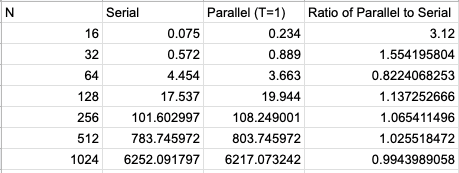
\includegraphics[width=\linewidth]{e2dat.png}\\
\null\\
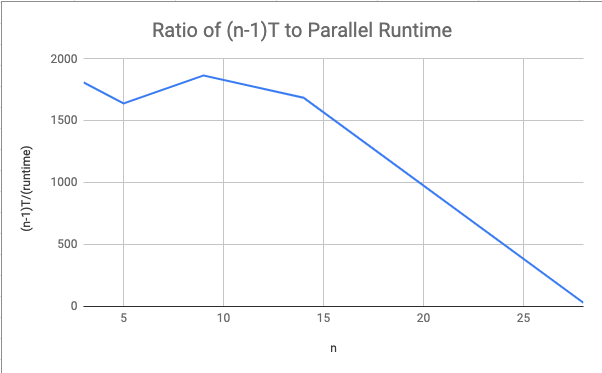
\includegraphics[width=\linewidth]{e2.png}\\
\textbf{\underline{Experiment 3}}\\
\textbf{\underline{Experiment 4}}\\
\textbf{\underline{Experiment 5}}

\end{adjustwidth}
\end{document}
